\documentclass[notes=show,beamer,compress]{beamer}

\usepackage{amssymb}
\usepackage{amsfonts}
\usepackage{amsmath}
\usepackage[absolute,overlay]{textpos}
\usepackage[english]{babel}
\usepackage[latin1]{inputenc}
\usepackage[T1]{fontenc}
\usepackage{graphicx}
\usepackage{bigstrut}
\usepackage{bbm}
\usepackage{txfonts}
\usepackage{array}

\mode<presentation> {
	\usetheme{Boadilla}
	\usecolortheme[RGB={103,102,204}]{structure}
	\useoutertheme{infolines}
	\setbeamercovered{transparent}
}


\setbeamercolor{bibliography entry title}{fg=black}
\setbeamercolor{bibliography entry author}{fg=black}
\setbeamercolor{subsection in toc}{fg=structure}
\setbeamercolor{palette primary}{bg=structure, fg=white}
\setbeamercolor{caption name}{fg=black} \setbeamersize{text margin
	left=.8cm} \setbeamersize{text margin right=1cm}
\hypersetup{linkbordercolor={1 0 0}} \setbeamertemplate{navigation
	symbols}{} \setbeamertemplate{headline}[default]

\setbeamertemplate{enumerate items}[default]


\title[]{Econometrics 2}
\subtitle{}
\author[Lychagin \& Mu\c{c}o]{Sergey Lychagin}
\institute[CEU]{CEU}
\date{Winter 2020}



\begin{document}

\frame{\titlepage}

\begin{frame}
	
	\begin{center}
		\Large Using IV when treatment effects are heterogeneous
	\end{center}
\end{frame}

\begin{frame}{Instrumental variables}
	\begin{itemize}
		\item Issue: outcome is correlated with treatment, $D_i$, even after conditioning on observables, $X_i$.
		\item IV ($Z_i$): exogenous and relevant.
		\item We use IV to isolate exogenous variation in $X_i$. Use this variation only to identify the causal effect of $X_i$ on $Y_i$.
		\item This works if the effect does not depend on $i$. But what if it does?
	\end{itemize} 
\end{frame}

\begin{frame}{Imbens-Angrist-Rubin potential outcome model}
	
	Stripped down version: no controls, binary instrument and treatment. There is a population of agents
	\begin{itemize}
		\item We randomly select agent $i$. This agent comes with $(Y_{0i}, Y_{1i})$ and $(D_{0i}, D_{1i})$ --- main outcome and treatment decision.
		\item We assign $Z_i=0,1$ -- an instrument -- independently of $(Y_{0i}, Y_{1i}, D_{0i}, D_{1i})$ (think of something that entices agents to take treatment)
		\item The treament is selected by the instrument: $D_i=D_{Z_ii}$
		\item The outcome is selected by the treatment: $Y_i=Y_{D_ii}$ (\textbf{implicit assumption: exclusion restriction})
	\end{itemize}
\end{frame}

\begin{frame}{Compliance types}
	Types, $T_i$:
	\begin{center}
		\begin{tabular}{|c|c|c|}
			\hline
			$D_{0i}$ & \multicolumn{2}{|c|}{$D_{1i}$} \\
			&      0      &        1         \\ \hline
			0     & never-taker &     complier     \\ \hline
			1     &   defier    &   always-taker   \\ \hline
		\end{tabular}
	\end{center}
	Variation in the instrument affects compliers and defilers. Never-takers and always-takers do not respond to $Z_i$.
	\begin{itemize}
		\item We don't observe one's type
		\item We observe which row one belongs to if $Z_i=0$
		\item We observe $i$'s column if $Z_i=1$
	\end{itemize}
	\textbf{No-defiance assumption} (or, monotonicity): $D_{1i}\geq D_{0i}$. 
\end{frame}

\begin{frame}{ATE for compliers?}
	Observables reveal the distribution of types:
	\begin{center}
		\begin{tabular}{|c|c|c|}
			\hline
			& \multicolumn{2}{|c|}{$Z_{i}$}                      \\ \hline
			$D_{i}$ &            0            &            1             \\ \hline
			0    & never-taker or complier &       never-taker        \\ \hline
			1    &      always-taker       & always-taker or complier \\ \hline
		\end{tabular}
	\end{center}
	\begin{itemize}
		\item Share of always-takers: $P_a = \Pr\{D_i=1|Z_i=0\}$
		\item Share of never-takers: $P_n = \Pr\{D_i=0|Z_i=1\}$
		\item The rest are compliers: $P_c = 1 - P_a - P_n$
	\end{itemize}
	This relies on $Z_i$ being independent of type.
\end{frame}

\begin{frame}{Outcomes for compliers}
	\begin{center}
		\begin{tabular}{|c|c|c|}
			\hline
			& \multicolumn{2}{|c|}{$Z_{i}$}                                      \\ \hline
			$D_{i}$ &                0                &                1                 \\ \hline
			0    & $Y_{0i}$ for $P_n$ never-takers &    $Y_{0i}$ for never-takers     \\
			&       and $P_c$ compliers       &                                  \\ \hline
			1    &   $Y_{1i}$ for always-takers    & $Y_{1i}$ for $P_a$ always-takers \\
			&                                 &       and $P_c$ compliers        \\ \hline
		\end{tabular}
	\end{center}
	Relate estimable statistics to potential outcomes
	\begin{align*}
		E[Y_{i}|Z_i=0, D_i=0] &= \frac{P_nE[Y_{0i}|T_i=n] + P_cE[Y_{0i}|T_i=c]}{P_n+P_c}\\
		E[Y_{i}|Z_i=1, D_i=0] &= E[Y_{0i}|T_i=n]
	\end{align*}
	This implies
	\begin{align*}
		E[Y_{0i}|T_i=c] &= \frac{P_c + P_n}{P_c}E[Y_{i}|Z_i=0, D_i=0]\\
		&- \frac{P_n}{P_c}E[Y_{i}|Z_i=1, D_i=0]
	\end{align*}
\end{frame}

\begin{frame}{Outcomes for compliers}
	\begin{center}
		\begin{tabular}{|c|c|c|}
			\hline
			& \multicolumn{2}{|c|}{$Z_{i}$}                                      \\ \hline
			$D_{i}$ &                0                &                1                 \\ \hline
			0    & $Y_{0i}$ for $P_n$ never-takers &    $Y_{0i}$ for never-takers     \\
			&       and $P_c$ compliers       &                                  \\ \hline
			1    &   $Y_{1i}$ for always-takers    & $Y_{1i}$ for $P_a$ always-takers \\
			&                                 &       and $P_c$ compliers        \\ \hline
		\end{tabular}
	\end{center}
	Similarly
	\begin{align*}
		E[Y_{1i}|T_i=c] &= \frac{P_c + P_a}{P_c}E[Y_{i}|Z_i=1, D_i=1]\\
		&- \frac{P_a}{P_c}E[Y_{i}|Z_i=0, D_i=1]
	\end{align*}
\end{frame}

\begin{frame}{Local average treatment effect}
	Definition: treatment effect for compliers
	\begin{align*}
		LATE = E[Y_{1i} - Y_{0i}|T_i=c]
	\end{align*}
	This can be expressed via observables using previous 3 slides. After some re-arrangements (check by substitution, use the rule of iterated expectations),
	\begin{align*}
		LATE = \frac{E[Y_i|Z_i=1] - E[Y_i|Z_i=0]}{E[D_i|Z_i=1] - E[D_i|Z_i=0]}
	\end{align*}
	We got the Wald estimator (IV with binary treatment \& instrument)! IV estimates LATE.\\\bigskip
	But what about always- and never-takers? Can't say anything about $Y_{0i}$ for the former, $Y_{i1}$ for the latter. Thus, $ATE$, $ATT$, $ATU$ are not point-identified in general.
\end{frame}

\begin{frame}{What if defiers exist?}
  Expand expectations in the numerator, make everything conditional on type:
	\begin{align*}
		E[Y_i|Z_i=1] - E[Y_i|Z_i=0] = &E[Y_{1i} - Y_{0i}|T_i=c]\Pr\{T_i=c\}\\ 
		&- E[Y_{1i} - Y_{0i}|T_i=d]\Pr\{T_i=d\}
	\end{align*}
	Denominator: $\Pr\{T_i=c\} - \Pr\{T_i=d\}$.
	
	Even if the effect is roughly similar for compliers and defiers, anything is possible: wrong sign, wrong magnitude.
\end{frame}

\begin{frame}{Extensions: multiple instruments?}
	LATE depends on the choice of instrument. For example
	\begin{itemize}
		\item Suppose we have two instruments for college education: $Z_1$, information treatment, and $Z_2$, a stipend
		\item Agents who respond to $Z_1$ may be very different from those who respond to $Z_2$
		\item If the effects are highly heterogeneous, don't be surprized if you get different IV estimates.
		\item Threat to external validity: LATE of education on earnings using an informational treatment IV may not be informative of returns to a stipend.
	\end{itemize}
\end{frame}

\begin{frame}{Extensions: multiple instruments?}
	
	What if estimates based on $Z_1$ and on $Z_2$ are very similar?
	\begin{itemize}
		\item If the respective compliers are \emph{very} different, this is a sign of little heterogeneity in TE
		\item If TEs don't vary across the agents, $LATE\approx TE$ for always- and never-takers
		\item $ATE\approx ATT \approx ATU \approx LATE$. 
	\end{itemize}
	How can one check if compliers for $Z_1$ and those for $Z_2$ are different?
\end{frame}

\begin{frame}{Multiple instruments: who are the compliers?}
	
	Do compliers for $Z_1$ differ from those for $Z_2$? Use observables $X_i$ to compare.\\\medskip
	
	Suppose $X_i$ is a dummy:
	\begin{align*}
		\Pr[X_i=1|T_i=c] &= \frac{\Pr\{T_i=c|X_i=1\}}{P_c}\Pr\{X_i=1\}\\
		&= \left(\Pr\{D_i=1|Z_i=1, X_i=1\} \right.\\
		&\phantom{=}- \left.\Pr\{D_i=1|Z_i=0, X_i=1\}\right)\frac{\Pr\{X_i=1\}}{P_c}
	\end{align*}
	Everything on the RHS can be approximated using the data. Compute this for $Z_1$ and $Z_2$ as IV\\\bigskip
	
	In the wage-college example, do stipend and information treatment compliers have similar incomes?
	
\end{frame}


%\begin{frame}{Extensions: multiple instruments}
%	
%	IV with multiple instruments:
%	\begin{itemize}
%		\item Can be represented as a weighted average of respective single-IV estimates
%		\item Thus, this is a weighted average of respective LATEs
%		\item Check Angrist and Imbens (1995) to learn more about the weights
%		\item Forget about standard tests of overidentifying restrictions -- they test if different IVs yield same results
%	\end{itemize}
%	
%\end{frame}
%
%
%\begin{frame}{Extensions: instrument of varying intensity}
%	
%	Think of the Mincer regression. Potential students are offered random (integer) stipends, $-\infty<Z_i<+\infty$. We may be able to get ATE now!
%	\begin{itemize}
%		\item Focus on students who get $Z_i=0$ and $Z_i=1$
%		\item Compliers at the baseline $Z=0$ --- choose college if offered $Z_i=1$, no college if offered $Z_i=0$.
%		\item IV for this subsample $=TE$ for compliers at $Z=0$
%		\item For any agent, there is a stipend $Z$ than makes him/her indifferent $\Rightarrow$ they are all compliers at some level of $Z$
%		\item By changing from $-\infty$ to $+\infty$, the instrument sweeps the entire population
%	\end{itemize}
%	We can find $LATE(Z)$ and $P_c(Z)$ for all levels of $Z$ and compute $ATE=\sum_Z LATE(Z)P_c(Z)$
%\end{frame}
%
%\begin{frame}{Extensions: controls}
%	
%	Conditional independence assumption: $(Y_{0i}, Y_{1i}, D_{0i}, D_{1i}) \Perp Z_i|X_i$. 
%	\begin{itemize}
%		\item For example, intention to treat is based on observables; take-up is endogenous
%		\item If $Z_i$ is independent of potential observables, using controls may still be beneficial: improving precision
%	\end{itemize}
%\end{frame}
%
%\begin{frame}{Extensions: controls}
%	
%	If $X$ takes a small number of values, or the sample is huge:
%	\begin{itemize}
%		\item Slice the sample based on $X$, run IV, get $LATE$ for each sample slice
%		\item Compute $LATE = \sum_X\Pr\{X_i=X\}LATE(X)$
%		\item Same can be done in one IV run: 
%		\begin{itemize}
%			\item Include $D$, dummies for the levels of $X$, their interactions on the RHS
%			\item Instrument $D$ with $Z$, interactions of $D$ and $X$ with interactions of $Z$ and $X$.
%		\end{itemize}
%	\end{itemize}
%	Not practical if $X$ is continuous or highly dimensional
%\end{frame}
%
%\begin{frame}{Extensions: controls}
%	
%	Same as above, but restrict the coefficient on $D_i$ to be the same for all $X$:
%	\begin{align*}
%		\text{1st stage:}\;D_i &= \gamma_X + \delta_XZ_i + v_i\; \text{for $i:X_i=X$}\\
%		\text{2nd stage:}\;Y_i &= \alpha_X + \beta D_i + u_i
%	\end{align*}
%	\begin{itemize}
%		\item Still many parameters to estimate, but less than before
%		\item Angrist and Imbens (1995): $\beta$ is a weighted average of $LATE(X)$. Higher predicted variance of $D_i$ -- higher weight (recall similar result in matching!).
%		\item Still too many parameters: $\alpha_X, \gamma_X, \delta_X$. Abadie (2003) addresses this, but his solution is not a standard IV.
%	\end{itemize}
%\end{frame}
%
%
\begin{frame}{IV --- concluding remarks}
	
	\begin{itemize}
		\item Things get really messy once TE heterogeneity is introduced
		\item Be careful extending your results to a different part of the population.
		\item E.g., you identify the effect of college education using an informational nudge as an instrument. 
		\item
		Your results may be misleading for statements about a tuition waiver policy. The value added of college may be different for people who respond to tuition waivers! 
	\end{itemize}
	
\end{frame} 

\begin{frame}
	
	\begin{center}
		\Large Starting your first research project
	\end{center}
\end{frame}

\begin{frame}{Things people value in research projects}
	What is usually met with interest?
	\begin{enumerate}
		\item Practical relevance: 
		
		When Y rises or falls, people are hurt or helped.
		\item Challenging common beliefs: 
		
		Prevailing wisdom says that X reduces Y, you find that X increases Y.
		\item Controversy: 
		
		Some argue one thing while other say another.
		\item Size: 
		
		Y is big (like the service sector) or common (like traffic jams).
	\end{enumerate}
		
\end{frame}

\begin{frame}{Things people value in research projects}
	
	Two dimensions of quality:
	\begin{enumerate}
		\item Internal validity: 
		
		Do we believe that we measure the true causal effect?
		\item External validity:
		
		Can we apply the results to other markets, time periods, countries?
	\end{enumerate}
	Different fields of economics put different emphasis on internal and external validity.
\end{frame}

\begin{frame}{How to start an empirical project}
	Several strategies:
	
	\medskip
	\textbf{Question-driven.} Pick a research theme, identify interesting questions. Work hard to get data.
	\begin{itemize}
		\item This is the 'proper' way, but can be risky (uninteresting results)
		\item{Data may be unavailable/expensive}
		\item{Identification is very hard; no good natural experiments}
		\item{Works well for: entrepreneurial types, people with access to funding}
	\end{itemize}
\end{frame}

\begin{frame}{How to start an empirical project}
	\textbf{``Freakonomics.''} Search for natural experiments. Then look for a dataset and a question.
	\begin{itemize}
		\item{Solid identification highly valued in the profession.}
		\item{Avoid narrow policy evaluation exercises (``Would my paper be interesting to a game theorist from Kazakhstan?'')}
		\item{Bad for personal marketing (``What exactly is your field?'')}
	\end{itemize}
\end{frame}

%

\begin{frame}{How to start an empirical project}
	\textbf{Data-driven.} Find rich data that few people used before. Then, find a question.
	\begin{itemize}
		\item{High sunk cost: collection/cleaning takes time. What if there is no good question?}
		\item{Before investing into data collection, ask yourself: What if I already have the ideal, cleaned dataset?}
		\item{Works well if: you already have some data.}
		\item{Uniqueness is a big plus. Quoting one editor:
			\begin{quote}
				[W]e all think that you have quite a unique data, and we are all confident that there exists a nice paper that can come out of these data.
		\end{quote}}
	\end{itemize}
\end{frame}

\begin{frame}{Workflow}
	Suppose you settled on the question, what's next? Write a research proposal (for yourself)
			\begin{itemize}
				\item What's the research question?
				\item Why is it interesting?
				\item How you are planning to answer it, intuitively?
				\item What data do you plan on using?
				\item What's new compared to the existing literature?
			\end{itemize}
	
	\bigskip
	
	Putting ideas into writing highlights weak points. Abandon/put aside hopeless projects early on!
\end{frame}

\begin{frame}{Workflow}
	At some point, the research proposal will morph into your paper's introduction.
	\bigskip
	
	As you go along, you may shift focus, switch to a different question. The process is iterative:
	\begin{itemize}
		\item Rewrite the introduction,
		\item Work on the analysis,
		\item Rewrite the introduction,
		\item Work on the analysis,
		\item $\dots$
		\item Cut unnecessary details, clean up the draft
	\end{itemize}
\end{frame}

\begin{frame}{Some examples from the past}
	Rozovskaya (2012) ``Can Observers Prevent Vote Fraud? Evidence from Russian Elections of 2011-2012
	in Moscow''
	
	\begin{itemize}
		\item Policy relevance?
		\item Controversial topic?
		\item Size?
	\end{itemize}
	Threat to identification: Observers are mostly sent to urban polling stations, places with higher perception of fraud.
	
	Research design --- natural experiment: observers are sent to polling stations in Moscow whose numbers end with a 0.
	
	\bigskip
	Lower votes for the ruling party, lower recorded turnout. Suggestive of ballot stuffing? The estimates are too low to question election outcome.

\end{frame}

\begin{frame}{Some examples from the past}
	Korganbekova (2014) ``The effect of hosting an Olympic Game on the performance of the National sports team at the following Olympics''
	
	\begin{itemize}
		\item Policy relevance?
		\item Controversial topic?
		\item Size?
	\end{itemize}
	Threat to identification: Olympic hosts are far from average. Selection on infrastructure, interest in sports?
	
	Research design --- diff-in-diff with a hand-picked control group:
	\begin{itemize}
		\item Countries who made bids to host in the same year,
		\item Countries who survived till the last round of selection.
	\end{itemize}
	The effect is $\approx 6$ medals, but the estimates are very noisy.
	
\end{frame}

\begin{frame}{Some examples from the past}
	Bardits (2016) ``The effect of the 2013 school centralization on school performance in Hungary''
	
	\begin{itemize}
		\item Policy relevance?
		\item Controversial topic?
		\item Size?
	\end{itemize}
	Mechanisms?
	\begin{itemize}
		\item Bureaucracy
		\item Change in funding
	\end{itemize}

	Threats to identification: Selection into treatment, by school, students, teachers.
\end{frame}

\begin{frame}{Some examples from the past}
	Research design --- diff-in-diff using school data
	\begin{itemize}
		\item All local public schools switch to central control in 2013
		\item Control group: church, private schools.
	\end{itemize}
	\begin{center}
	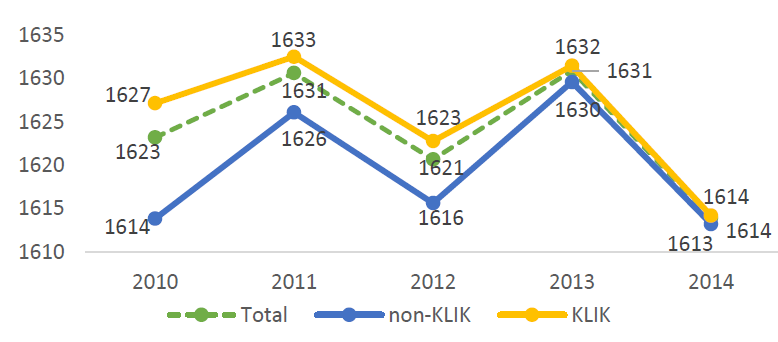
\includegraphics[width=3in]{graphs/bardits.png}
	\end{center}
	External validity? The more we can say about the mechanism, the broader the implications. Can't say much here.
\end{frame}

\end{document}
